\cleardoublepage

{
    \sectionnonum{附~~~~录}

    \appendixsubsecmajornumbering

    \subsection{Vulkan 中的稀疏资源}
    \label{appendix:sparse}

    在 Vulkan 中,稀疏资源扩展将资源划分为四种类型。这里我们以缓冲区为例,简要介绍这四类资源的差异和应用场景。

    \subsubsection{Vulkan 中的缓冲区类型}

    \begin{figure}[htbp]
        \centering
        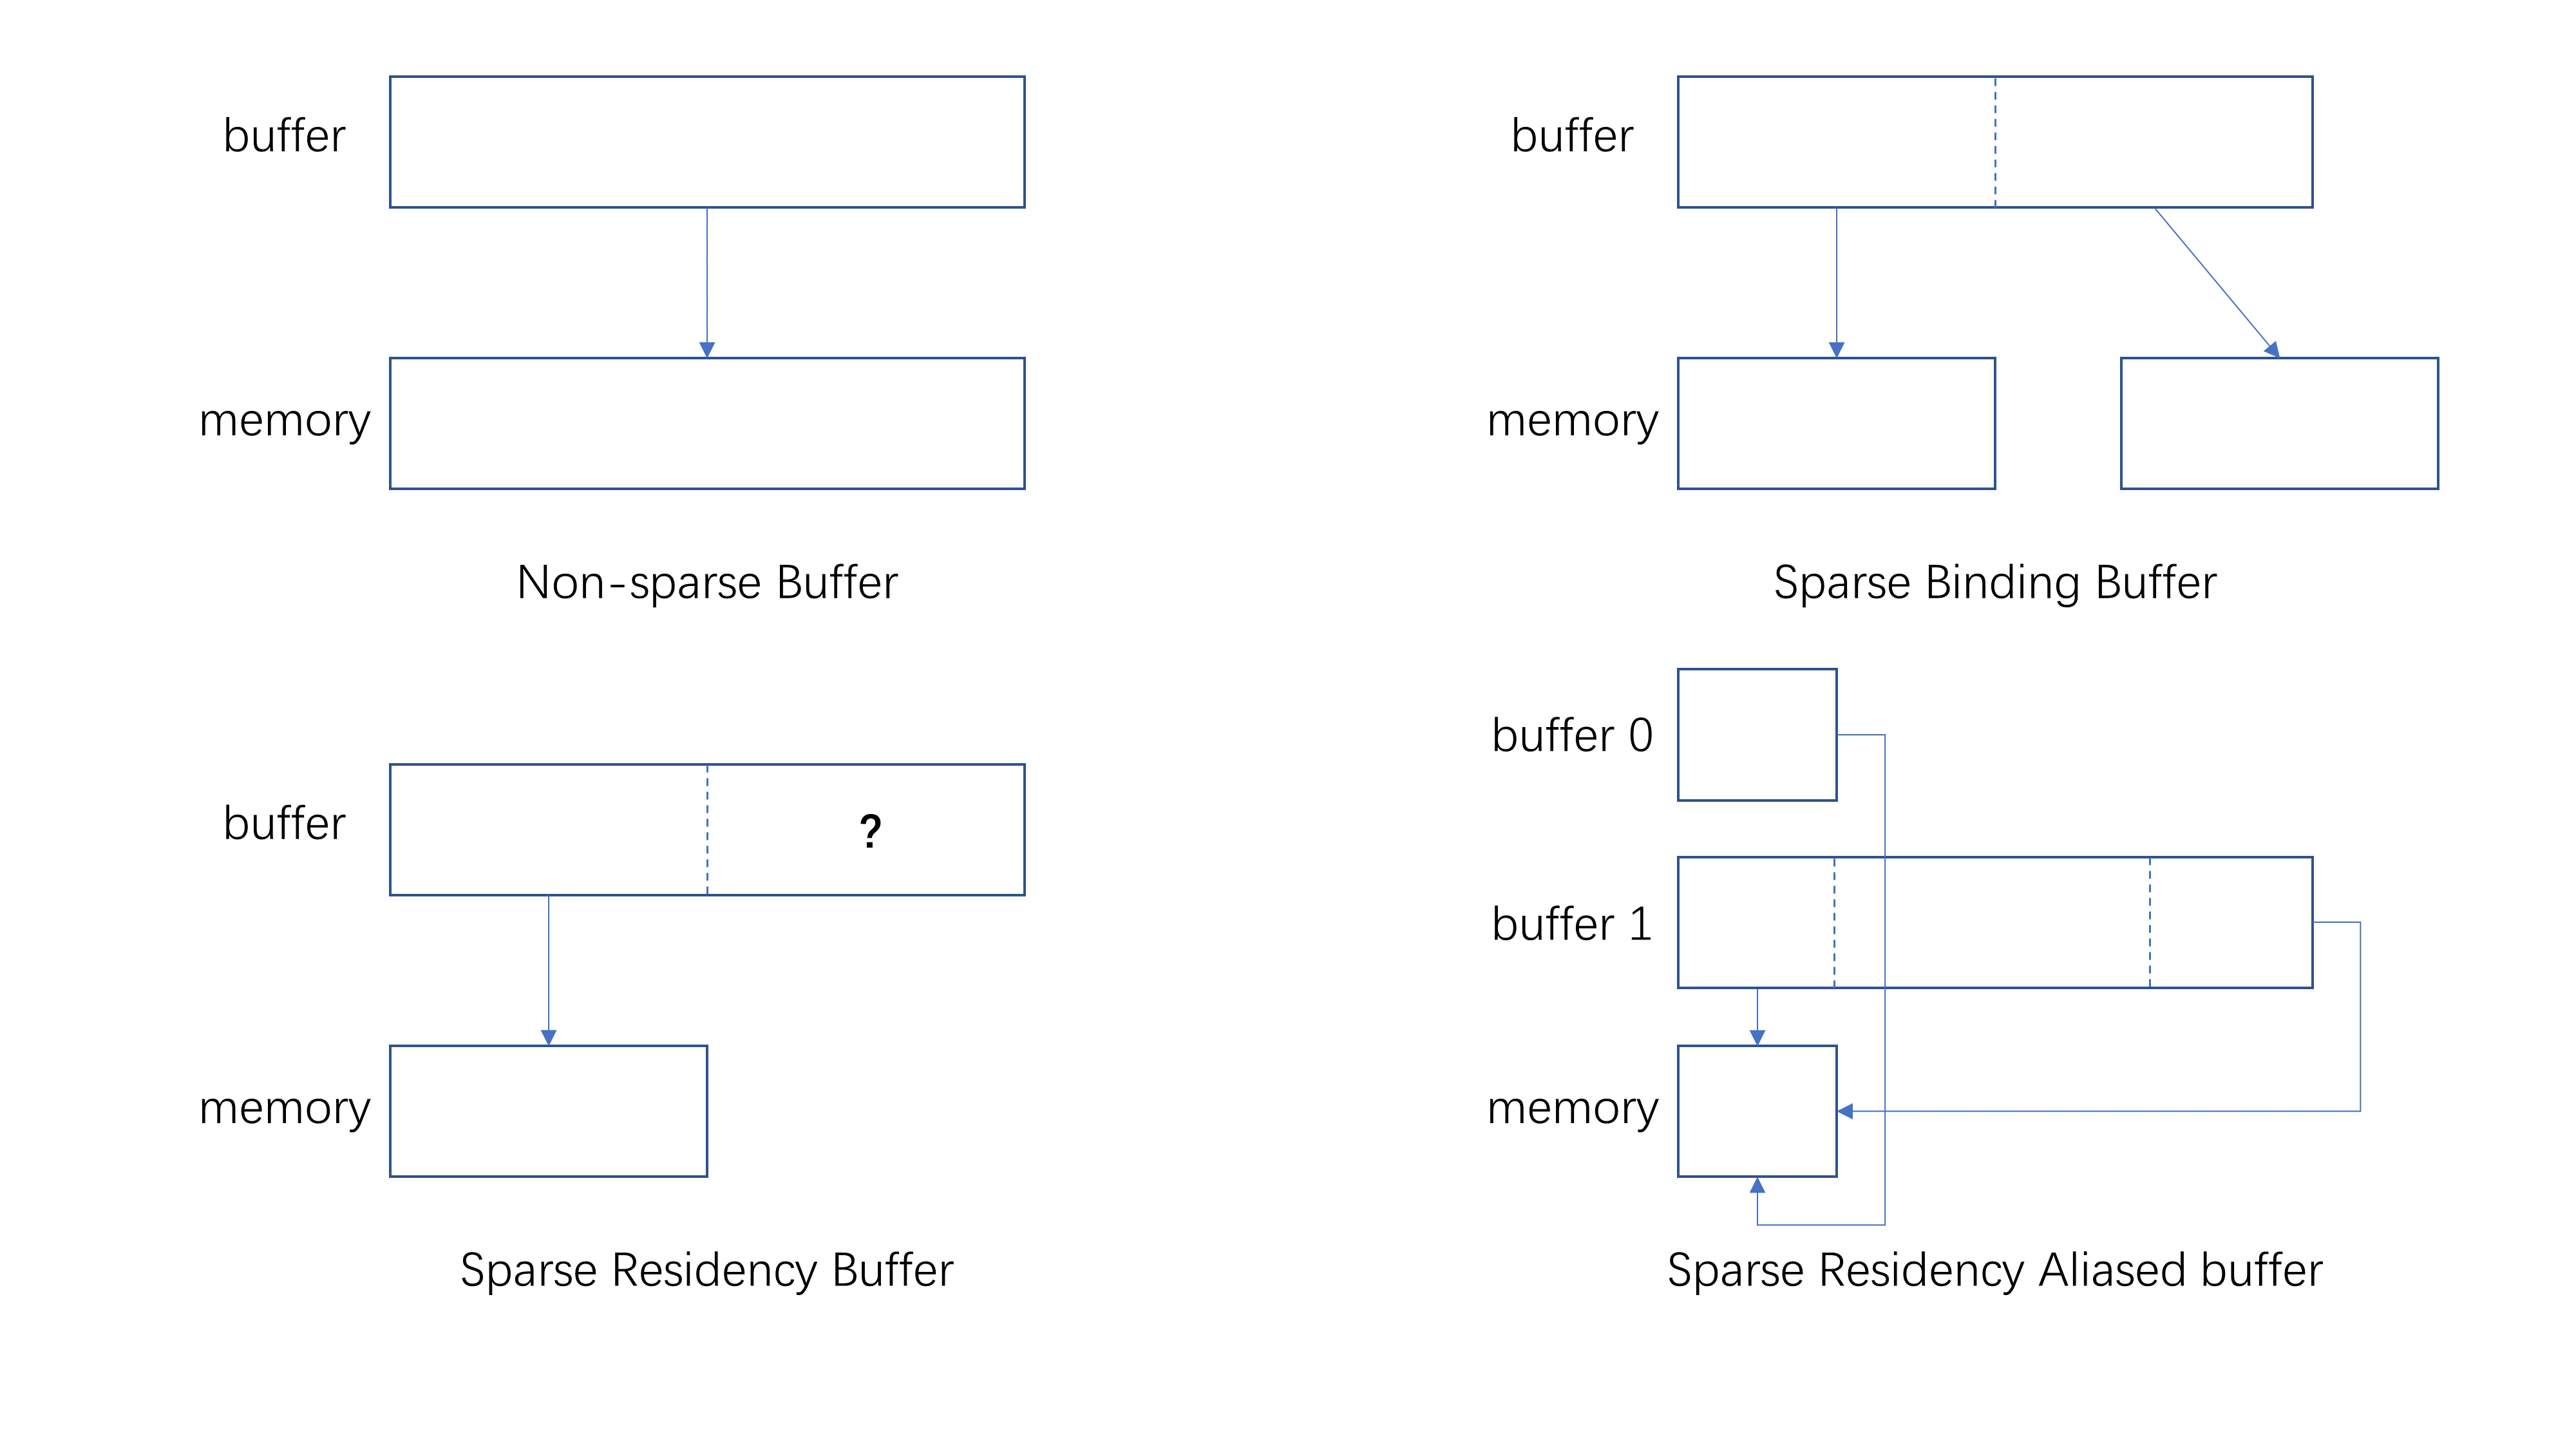
\includegraphics[width=\linewidth]{sparse.png}
        \caption{\label{fig:sparse}Vulkan 中不同缓冲区类型的内存绑定方式}
    \end{figure}
    
    如\autoref{fig:sparse}所示,Vulkan 根据是否支持稀疏绑定(sparse binding)和稀疏驻留(sparse residency),将缓冲区分为以下四类:

    \begin{itemize}
        \item \textbf{Non-sparse Buffer}:默认的缓冲区类型,需在创建后绑定到某个显存,绑定后不可更改。其简单但缺乏灵活性,无法满足动态资源调度的需求。
        
        \item \textbf{Sparse Binding Buffer}:支持以页为单位绑定显存,允许在运行时修改缓冲区和显存之间的绑定关系。但缓冲区的所有区域都必须完成绑定,否则行为未定义。
        
        \item \textbf{Sparse Residency Buffer}:在 Sparse Binding Buffer 的基础上引入了稀疏驻留机制。允许缓冲区部分区域未绑定显存,如果访问了未绑定的区域,系统将返回默认值而不会产生非法访问。这类缓冲区非常适合按需加载,支持更大规模的数据组织。
        
        \item \textbf{Sparse Residency Aliased Buffer}:在 Sparse Residency Buffer 的基础上进一步允许多个资源共享同一组显存页,适合需要显存复用的高级应用场景,但需要开发者额外管理资源之间的别名冲突,使用复杂。
    \end{itemize}

    \subsubsection{本项目的选择与理由}
    本项目采用了 Sparse Residency Buffer 来存储大规模工业场景中的几何数据,其主要优势包括:

    \begin{itemize}
        \item \textbf{支持细粒度的显存控制}:缓冲区与显存不再是一对一的关系,能够将缓冲区划分成页进行管理,大大提高了资源调度的灵活性;
        
        \item \textbf{支持动态换绑}:允许在运行时更换显存页的绑定位置,适配页表中的换页操作;

        \item \textbf{支持按需加载}:缓冲区的部分区域可以不绑定显存页,仅在需要渲染对应数据时才绑定,减少了不必要的显存占用;
        
        \item \textbf{访问未绑定区域安全}:当部分区域尚未绑定显存页时,GPU 访问这些区域也不会触发未定义行为导致系统崩溃,仅会返回默认值,这为延迟加载提供了容错能力,保证了系统的鲁棒性。
    \end{itemize}

    综上所述,Sparse Residency Buffer 在灵活性与鲁棒性之间达到了较好的平衡,是本项目实现高效流式加载和显存管理的关键基础设施。

    \subsection{源代码清单}

    本项目的全部源代码已托管于 GitHub 开源仓库中,地址如下:

    \begin{itemize}
    \item \url{https://github.com/F-Fumino/Xihe}
    \end{itemize}

    该仓库包含渲染引擎的完整实现,包括基于任务着色器的簇剔除流程、流式加载调度机制、LOD 管理等模块。访问时间为 2025 年 5 月。

    % End of appendix
    \removeappendixsubsecmajornumbering
}